
\documentclass[a4paper, 12pt]{article}

%\usepackage{dtma}
\usepackage[fleqn]{amsmath}
\usepackage{geometry}
\usepackage{fancyhdr}
\usepackage{graphicx}
\usepackage{lastpage}

% Set up spaces and alignment the way I like it ------------------------------------------
\geometry{includemp}
\geometry{headheight=10mm, headsep=10mm, bottom=15mm, footskip=15mm, marginparwidth=18mm, marginparsep=5mm}
\geometry{voffset=-6mm, hoffset=-5mm, lmargin=35mm, rmargin=5mm}
\setlength{\headwidth}{\textwidth}
\setlength{\parindent}{0mm}			% Paragraph indentation
\setlength{\parskip}{5mm}			% Paragraph spacing
\renewcommand{\baselinestretch}{1.0}		% Line spacing
\setlength{\mathindent}{10 mm}
%-----------------------------------------------------------------------------------------

% Set up the banner headline--------------------------------------------------------------
\newcommand{\banner}{\relax}
\newcommand{\mybanner}[1]{\renewcommand{\banner}{#1}}

\mybanner{%
	\textbf{Derivation of the Poisson distribution from the Binomial distribution}
	\newline
	From M248 Screencast 3.2, with additional notes from MST124
}
\pagestyle{fancy}
\lhead{\textrm{\banner}}
\cfoot{ \ Page \thepage \ of \pageref{LastPage}}
%-----------------------------------------------------------------------------------------

% For random variable "is distributed as" with overset------------------------------------
\makeatletter
\newcommand{\distas}[1]{\mathbin{\overset{#1}{\kern\z@\sim}}}% default spacing
\newsavebox{\mybox}\newsavebox{\mysim}
\newcommand{\distras}[1]{%
	\savebox{\mybox}{\hbox{\kern3pt$\scriptstyle#1$\kern3pt}}%
	\savebox{\mysim}{\hbox{$\sim$}}%
	\mathbin{\overset{#1}{\kern\z@\resizebox{\wd\mybox}{\ht\mysim}{$\sim$}}}% mod space if overset large
}
\makeatother

% Set default to left for margin notes:
\reversemarginpar				% Sets default to left margin for margin notes
%-----------------------------------------------------------------------------------------

% Establish counter for equation numbering------------------------------------------------
\newcounter{QEq}				% Comment out if using dtma.sty
\numberwithin{equation}{QEq}	% For n.1, n.2, n.etc (I think)
%-----------------------------------------------------------------------------------------
% Add these 2 lines before each new question (but not subquestions)
%  \refstepcounter{QEq}		% or \stepcounter{QEq}
%  \setcounter{equation}{0}
%-----------------------------------------------------------------------------------------

% If you're sitting comfortably, now we'll begin------------------------------------------
% ("Listen with mother" from when I was a kid

\begin{document}
\refstepcounter{QEq}
\setcounter{equation}{0}
	
The Binomial distribution \(X \sim B(n,p) \text{, } x=0,1,2, \ldots\) has parameters \(n\) and \(p\) and has probability mass function:
\begin{equation}
	p(x) = \binom{n}{n-x}\,p^{x}\,(1-p)^{n-x} \label{eq:Bpmf}
\end{equation}
When we start to consider the Poisson distribution, we shall start using the Binomial p.m.f. \eqref{eq:Bpmf} but substitute the Poisson parameter \(\lambda \; (=np)\).

\vspace{10mm}

\textbf{\underline{\(P(X=0)\)}}

Let us begin with the Binomial probability for \(P(X=0)\):
\refstepcounter{QEq}
\begin{align}
	p(0) &= \binom{n}{n-0}\,p^{0}\,(1-p)^{n-0} \nonumber \\
	&= 1 \times 1 \times (1-p)^{n} \nonumber \\
	&= (1-p)^{n} \nonumber 
	\intertext{Expressed usuing the parameter of the Poisson distribution \(\lambda = np\):}
	p(0) &= \left(1-\frac{\lambda}{n}\right)^n \label{eq:Ppmf0}
\end{align}

\vspace{5mm}

Before we proceed any further, it is helpful to consider how we can arrive at a formula for the poisson distribution that includes a term containing \(e^{-\lambda}\). We need to use techniques learned in MST124, namely the use of the binomial expansion to expand \((a+b)^n\) and then to link this to the Taylor series expansions of the function \(f(x) =e^x\).

We shall return to \(P(X=0)\) later.

\vspace{10mm}

\textbf{\underline{Binomial expansion}}

The binomial expansion is:
\refstepcounter{QEq}
\begin{align}
	(a+b)^n &= \binom{n}{0}a^{n}\,b^{0} + \binom{n}{1}a^{n-1}\,b^{1} + \ldots + \binom{n}{n-1}a^{1}\,b^{n-1}  + \binom{n}{n}a^{0}\,b^{n} \label{eq:binexp} \\
	\intertext{Let \(a=1\) and \(b=x\):}
	&= \binom{n}{0}\,x^{0} + \binom{n}{1}\,x^{1} + \binom{n}{3}\,x^{3} + \dots + \binom{n}{n}\,x^{n} \nonumber \\
	&= \frac{n!}{0! (n-0)!}\,x^{0} + \frac{n!}{1! (n-1)!}\,x^{1} + \ldots + 
	\frac{n!}{(n-1)!\,1!}\,x^{n-1} + \frac{x^{n}}{n!} \nonumber \\
	&= \frac{n!}{(n-0)!}\,\frac{x^{0}}{0!} + \frac{n!}{(n-1)!}\,\frac{x^{1}}{1!} + \ldots + \frac{n!}{1!}\,\frac{x^{(n-1)}}{(n-1)!} + \frac{x^{n}}{n!} \nonumber \\
	&= 1 + nx + n(n-1)\frac{x^{2}}{2!} + n(n-1)(n-2)\frac{x^{3}}{3!} + \dots + \frac{x^{n}}{n!} \nonumber
	\intertext{Let \(x = \frac{z}{n}\) with \(n \rightarrow \infty\):}
	(a+b)^n &= 1 + z + \frac{z^2}{2!} + \frac{z^3}{3!} + \dots + \frac{z^n}{n!} \label{eq:bintaylor} 
\end{align}

\vspace{10mm}

\textbf{\underline{Taylor series}}

The function \(f(z) = e^z\) can be repeatedly differentiated and for each iteration \(f^{(k)}(z) = e^z\). Therefore, we can approximate the function by Taylor expansion. The Taylor polynomial about point  \(a\) is:
\refstepcounter{QEq} %\nonumber \label{eq:} %% place where integer increments are needed
\begin{align}
	p(z) &= f(a) + f'(a)(z-a) + \frac{f''(a)}{2!}(z-a)^2 + \frac{f^{(3)}(a)}{3!}(z-a)^3 + \nonumber \\
	& \qquad \qquad \qquad \qquad \qquad \qquad \qquad \qquad \qquad \qquad \ldots + \frac{f^{(n)}(a)}{n!}(z-a)^n \nonumber \\
	\intertext{When  \(a=0\):}
	p(z) &= f(0) + f'(0)z + f''(0)\frac{z^2}{2!} + f^{(3)}(0)\frac{z^3}{3!} + f^{(n)}(0)\frac{z^n}{n!} \nonumber \\
	&= 1 + z  + \frac{z^2}{2!} + \frac{z^3}{3!} + \ldots + \frac{z^n}{n!} \label{eq:ptaylor}
\end{align}
This is the Taylor series which approximates the function \(f(z) = e^z\). This allows us to recognise that the binomial expansion of \(\left(1+\frac{z}{n}\right)^n\) tends to \(e^z\) as \(n \rightarrow \infty\).

Replacing \(z\) with \(-\lambda\), we get:
\begin{equation}
\left(1-\frac{\lambda}{n}\right)^n = e^{-\lambda} \qquad \text{for large } n \label{eq:e^lamba}
\end{equation}

\newpage{}

\textbf{\underline{Return to \(P(X=0)\)}}

Now that we have seen why \(\left(1-\frac{\lambda}{n}\right)^n = e^{-\lambda}\) for large \(n\) we can resume our consideration of the probability that \(P(X=0)\). We can restate that:
\refstepcounter{QEq} %\nonumber \label{eq:} %% place where integer increments are needed
\begin{align}
	p(0) &= \left(1-\frac{\lambda}{n}\right)^n \nonumber \\[2mm]
	&= e^{-\lambda} \label{eq:p0}
\end{align}

\vspace{10mm}

\textbf{\underline{For \(P(X > 0)\)}}

We calculate each new probability \(P(X=x)\) from the previous probability \(P(X=x-1)\):
\refstepcounter{QEq} %\nonumber \label{eq:} %% place where integer increments are needed
\begin{align}
	\frac{p(x)}{p(x-1)} &= 	\frac{\binom{n}{x}\,p^x\,(1-p)^{n-x}}{\binom{n}{x-1}\,p^{x-1}\,(1-p)^{n-x+1})} \label{eq:pxoverx-1} \\[2mm]
	&= \frac{\binom{n}{x}}{\binom{n}{x-1}} 
	\times \frac{p^x}{p^{x-1}} 
	\times \frac{(1-p)^{n-x}}{(1-p)^{n-x+1}}\nonumber 
	\intertext{But:}
	\frac{p^x}{p^{x-1}} &= \frac{p^x}{p^x\,p^{-1}} \nonumber \\[2mm]
	&= p \label{eq:p} \\[2mm]
	\intertext{Similarly:}
	\frac{(1-p)^{n-x}}{(1-p)^{n-x+1}} &= \frac{(1-p)^{n-x}}{(1-p)^{n-x}\,(1-p)^1} \nonumber \\[2mm]
	&= \frac{1}{1-p} \label{eq:1-p}
	\intertext{So:}
	\frac{p(x)}{p(x-1)} &= 	\frac{\binom{n}{x}\,p}{\binom{n}{x-1}\,(1-p)} \nonumber 
\end{align}

We can also simplify the binomial coefficients:
\begin{align}
	\frac{\binom{n}{x}}{\binom{n}{x-1}} &= 
	\frac{n!}{x! \, (n-x)!} \div \frac{n!}{(x-1)! \, (n-x+1)!} \nonumber \\[2mm]
	&= \frac{(x-1)!}{x!} \times \frac{(n-x+1)!}{(n-x)!} \nonumber \\[2mm]
	&= \frac{1}{x}\,(n-x+1) \label{eq:n-x+1}
\end{align}

\newpage{}

Replacing the terms in equation \eqref{eq:pxoverx-1}:
\begin{equation}
	\frac{p(x)}{p(x-1)} = \frac{(n-x+1)}{x} \times \frac{p}{(1-p)}	\label{eq:Eq2}
\end{equation}
Substituting \(p=\frac{\lambda}{n}\) and also \(1-p=1-\frac{\lambda}{n} \;\;(=1-\frac{\lambda}{n})\), we get:
\begin{align*}
	\frac{p}{1-p} &= \frac{\lambda}{n} \div \frac{n-\lambda}{n} \\[2mm]
	&= \frac{\lambda}{n} \times \frac{n}{n-\lambda} \\[2mm]
	&= \frac{\lambda}{n-\lambda}
\end{align*}

Equation \eqref{eq:Eq2} becomes:
\[
	\frac{p(x)}{p(x-1)} = \frac{n-x+1}{x} \times \frac{\lambda}{n-\lambda}	%create label "Equation (3)"
\]

Expressing this in terms of \(p(x)\) gives:
\[
	p(x) = \frac{n-x+1}{n-\lambda} \times \frac{\lambda}{x} \times p(x-1)
\]
As \(n\) becomes large, \(\frac{n-x+1}{n-\lambda} \rightarrow 1\)

\vspace{10mm}

\textbf{\underline{Bringing it all together}}

Gathering together the expressions that we have obtained for the probabilities of \(P(X=0)\) and \(P(X=x)\), we have a system of equations that can approximate the Binomial distribution with parameters \(n\) and \(\frac{\lambda}{n}\), which is \(X \sim B(n, \frac{\lambda}{n})\) with \(x=1,2,3,\ldots\) for a large sample size.

Using the system of equations to evaluate \(P(X=1)\):
\begin{align*}
	p(1) &= \frac{\lambda}{1} \, p(0) \\[2mm]
	&= \frac{\lambda}{1} \, e^{-\lambda}
\end{align*}

Using a similar tachnique to evaluate \(P(X=2)\) and \(P(X=3)\):
\begin{align*}
	p(2) &= \frac{\lambda}{2} \, p(1) \\[2mm]
	&= \frac{\lambda^2}{2 \times 1} \, e^{-\lambda} \\[2mm]\\
	p(3) &= \frac{\lambda}{3} \, p(1) \\[2mm]
	&= \frac{\lambda^3}{3 \times 2 \times 1} \, e^{-\lambda}
\end{align*}

From this pattern, we can see that the probability mass function is:
\refstepcounter{QEq} %\nonumber \label{eq:} %% place where integer increments are needed
\begin{equation}
p(x) = \frac{\lambda^x \, e^{-\lambda}}{x!} \qquad x=1,2, \dots \label{eq:bingo}
\end{equation}
Thus, we have shown that the Poisson distribution is derived from the Binomial distribution with parameters \(n\) and \(\frac{\lambda}{n}\) for a large sample size, \(n\).

\vspace{40mm}

\textbf{\underline{Appendix: extracts from MST124}}

\begin{figure}[h!]
\centering
	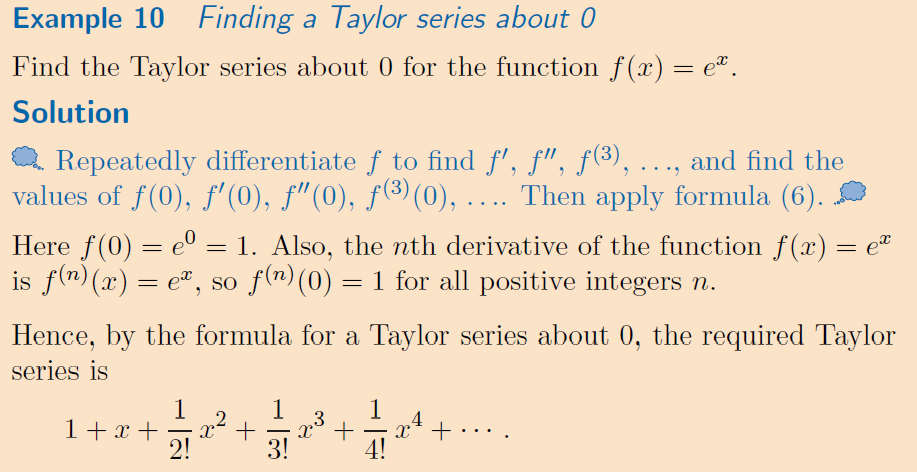
\includegraphics[scale=0.68]{TaylorSeries.png} \\
	\caption{MST124; Book D; Example 10; Page 138}
\end{figure}

\vspace{15mm}

When calculating the Taylor series for function \(f(x)=e^x\), we use repeated differentiation of the function. For \(e^x\):
\[
	f(x)=e^x \quad f'(x)=e^x \quad f''(x)=e^x \quad f^{(3)}(x)=e^x \quad f^{(4)}(x)=e^x \quad \text{etc.}
\]

The derivation of the Taylor polynomial is:
\begin{figure}[h!]
\centering
	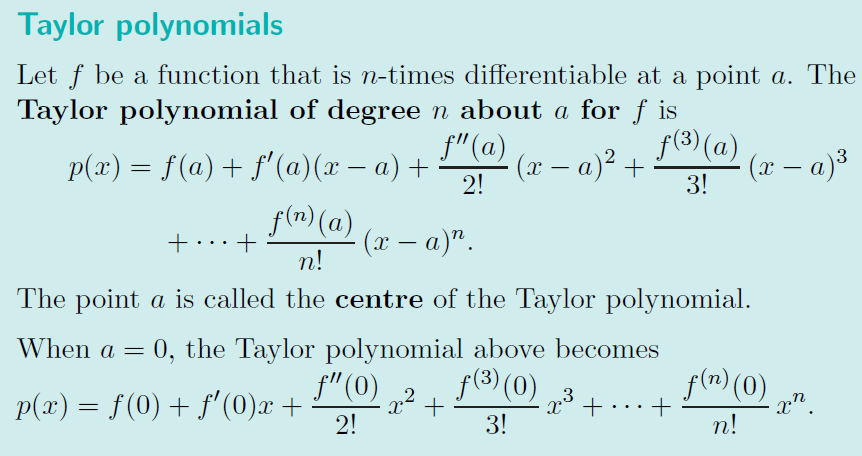
\includegraphics[scale=0.72]{TaylorPolynomial.png} \\
	\caption{MST124; Book D; page 121}
\end{figure}

\vspace{15mm}

\begin{figure}[h!]
\centering
	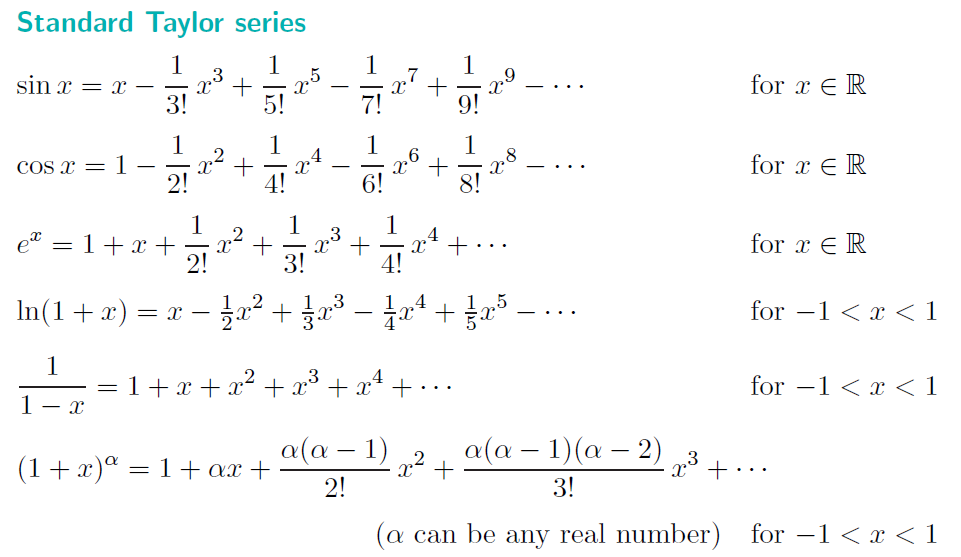
\includegraphics[scale=0.72]{TaylorSeries_HB.png} \\
	\caption{MST124; Handbook; page 8}
\end{figure}

\end{document}